% Activate the following line by filling in the right side. If for example the name of the root file is Main.tex, write
% "...root = Main.tex" if the chapter file is in the same directory, and "...root = ../Main.tex" if the chapter is in a subdirectory.
 
%!TEX root =  

\chapter[Monte Carlo]{Monte Carlo}

In order to understand both the signal and backgrounds better, Monte Carlo (MC) datasets are computer-
generated simulation events that allow a physicist to develop and validate an analysis.  The generation and refinement of MC 
algorithms and datasets could be a thesis in its own right, but this section will touch on some of 
the most relevant features of the MC datasets used in this algorithm.


\section{MC Creation Procedure}
\label{sec:mc-gen-overview}
MC events are generally created in four major steps.  
\begin{enumerate}
    \item First, the generator uses quantum field theory to simulate the hard 
    scatter, generally starting with a proton and ending with all final-state particles.  
    \item Then those particles are handed off to a dedicated algorithm that simulates 
    how they would shower and hadronize, where appropriate.  
    \item Next, the resulting particles from the first two steps are put 
    into a detector simulation, which uses information on the detector materials and geometry 
    to understand how the particles evolve as they travel through the ATLAS detector.  
    \item The detector's response to the particles is simulated in a 
    digitization and reconstruction step, so that the final output is an event that 
    looks similar to how a ``real'' event of that type might look in the ATLAS detector. 
\end{enumerate} 

\section{Signal Monte Carlo}
MadGraph \cite{MadGraph} is used to generate the signal MC, with showering and 
hadronization done in Pythia6 \cite{Pythia6}.  Madgraph uses a 5 flavor scheme PDF 
(parton distribution function), meaning that it models $b$-quarks in the proton as 
well as the more common light flavor (up, down, charm and strange quarks, 
and gluons).  In addition to the Higgs production with the associated $b$-quark and 
the Higgs decay, there can also be extra jets in the event from initial state radiation (ISR) 
and/or final state radiation (FSR).  We allow up to two additional partons per 
event in the signal MC; the generation and cross-section calculations tend to be more 
accurate for higher numbers of extra partons allowed but at the cost of exponentially slower and more 
complicated generation times (Table~\ref{tab:mg_times}).  We found two jets to be a reasonable cutoff where the distributions did 
not seem to be affected by allowing for higher numbers of extra partons, but the generation 
time was still acceptably quick.  The matching scale for knitting together the hard scatter
calculations in MadGraph with the Pythia hadronization and showering was set to 20 GeV.

%--------------------------------------------------------
\begin{table}
   \caption{The cross sections and generation times for MadGraph signal MC as a function
   of number of additional partons allowed, for 0-3 partons.  There is approx. 2.5\%
   difference between the 3-parton and 4-parton cross sections, which comes at a cost
   of hours of CPU time.  The times quoted here are for generating 10,000 events per 
   sample, before hadronization. \label{tab:mg_times}} 
    \center
    \begin{tabular}{ c c c } \hline\hline
    Process & $\sigma [pb]$ & time \\ \hline
    $pp\rightarrow h^0b + <=0j$ & 1.843e-5 $\pm$ 4.2e-08 & seconds \\
    $pp\rightarrow h^0b + <=1j$ & 2.555e-5 $\pm$ 7.3e-08 & seconds \\
    $pp\rightarrow h^0b + <=2j$ & 2.762e-5 $\pm$ 8.2e-08 & minutes \\
    $pp\rightarrow h^0b + <=3j$ & 2.83e-5 $\pm$ 9e-08 & $~$ 4 hours \\
    \end{tabular}
\end{table}

%--------------------------------------------------------



%--------------------------------------------------------
\begin{table}
   \caption{The signal MC samples and their parameters. \label{tab:sig_mc_parameters} }
    \center
    \begin{tabular}{ c c c } \hline\hline
    Dataset ID & mass (GeV) & width (GeV) \\ \hline
    181120     & 250        & 1.68682 \\
    181121     & 280        & 1.92318 \\
    181122     & 310        & 2.50849 \\
    181123     & 350        & 3.23507 \\
    181124     & 400        & 3.93561 \\
    181125     & 450        & 4.71906 \\
    181126     & 500        & 5.59454 \\
    181127     & 550        & 6.84368 \\
    181128     & 600        & 8.11044 \\
    181129     & 650        & 9.26688 \\
    181130     & 700        & 10.3760 \\
    181131     & 800        & 12.5049 \\ \hline
    \end{tabular}
\end{table}

%--------------------------------------------------------




The Madgraph signal generation is done for 12 different mass points, spanning 250-800 GeV
. Below 250 GeV, the daughter $b$-jets from the Higgs tend to be 
too low-$p_T$ to fire the trigger, while above 800 GeV SUSY 
becomes less appealing theoretically.  Since both the production and decay of $bH\rightarrow bbb$ 
happen via SM interactions, with SUSY only becoming relevant for increasing the production cross section and 
widening the inherent width of the $A/H$ distributions, the signal generation can 
be done by using an SM $bH\rightarrow bbb$ production model but with a 
modified Higgs width.  There are 300,000 signal events generated for each mass point.

% ATF-II source: http://iopscience.iop.org/1742-6596/396/2/022031
The detector simulation for the signal MC was done using AtlFast-II (AFII) \cite{ATF2}, 
a modified version of Geant4 \cite{Geant4-1, Geant4-2} designed 
to cut down on the considerable time required for simulating particle interactions with the detector, especially 
showers in the calorimeter.  AFII does full simulation of the inner detector and tracking, but 
uses frozen shower shapes taken from a large collection of pre-generated samples to speed up 
the simulation.  After simulation, the digitization and reconstruction are handled by the ATLAS standard algorithms 
in the ATHENA framework, as is standard for all ATLAS MC.    



%https://indico.cern.ch/event/235341/contribution/1/material/slides/0.pdf
\subsection{Generator Comparisons}
In addition to MadGraph, Sherpa and Pythia are some other signal MC generators that 
were studied.  As an NLO generator, MadGraph has the advantage over Pythia (an LO generator) of including
more Feynman diagrams that are important to this analysis.  Sherpa has the disadvantage that
the Higgs is not stored in the truth table, which makes it impossible to positively
disambiguate between Higgs daughter $b$-quarks and associated $b$-quarks.  Sherpa
also shows kinematic differences from both MadGraph and Pythia in the $p_T$ of the truth
jets (Figure~\ref{fig:sig_gen_compare}), which of course then also propagates through to the $m_{bb}$ distribution
(Figure~\ref{fig:mbb_sherpa_pythia_madgraph}).


\begin{figure}
  \center
  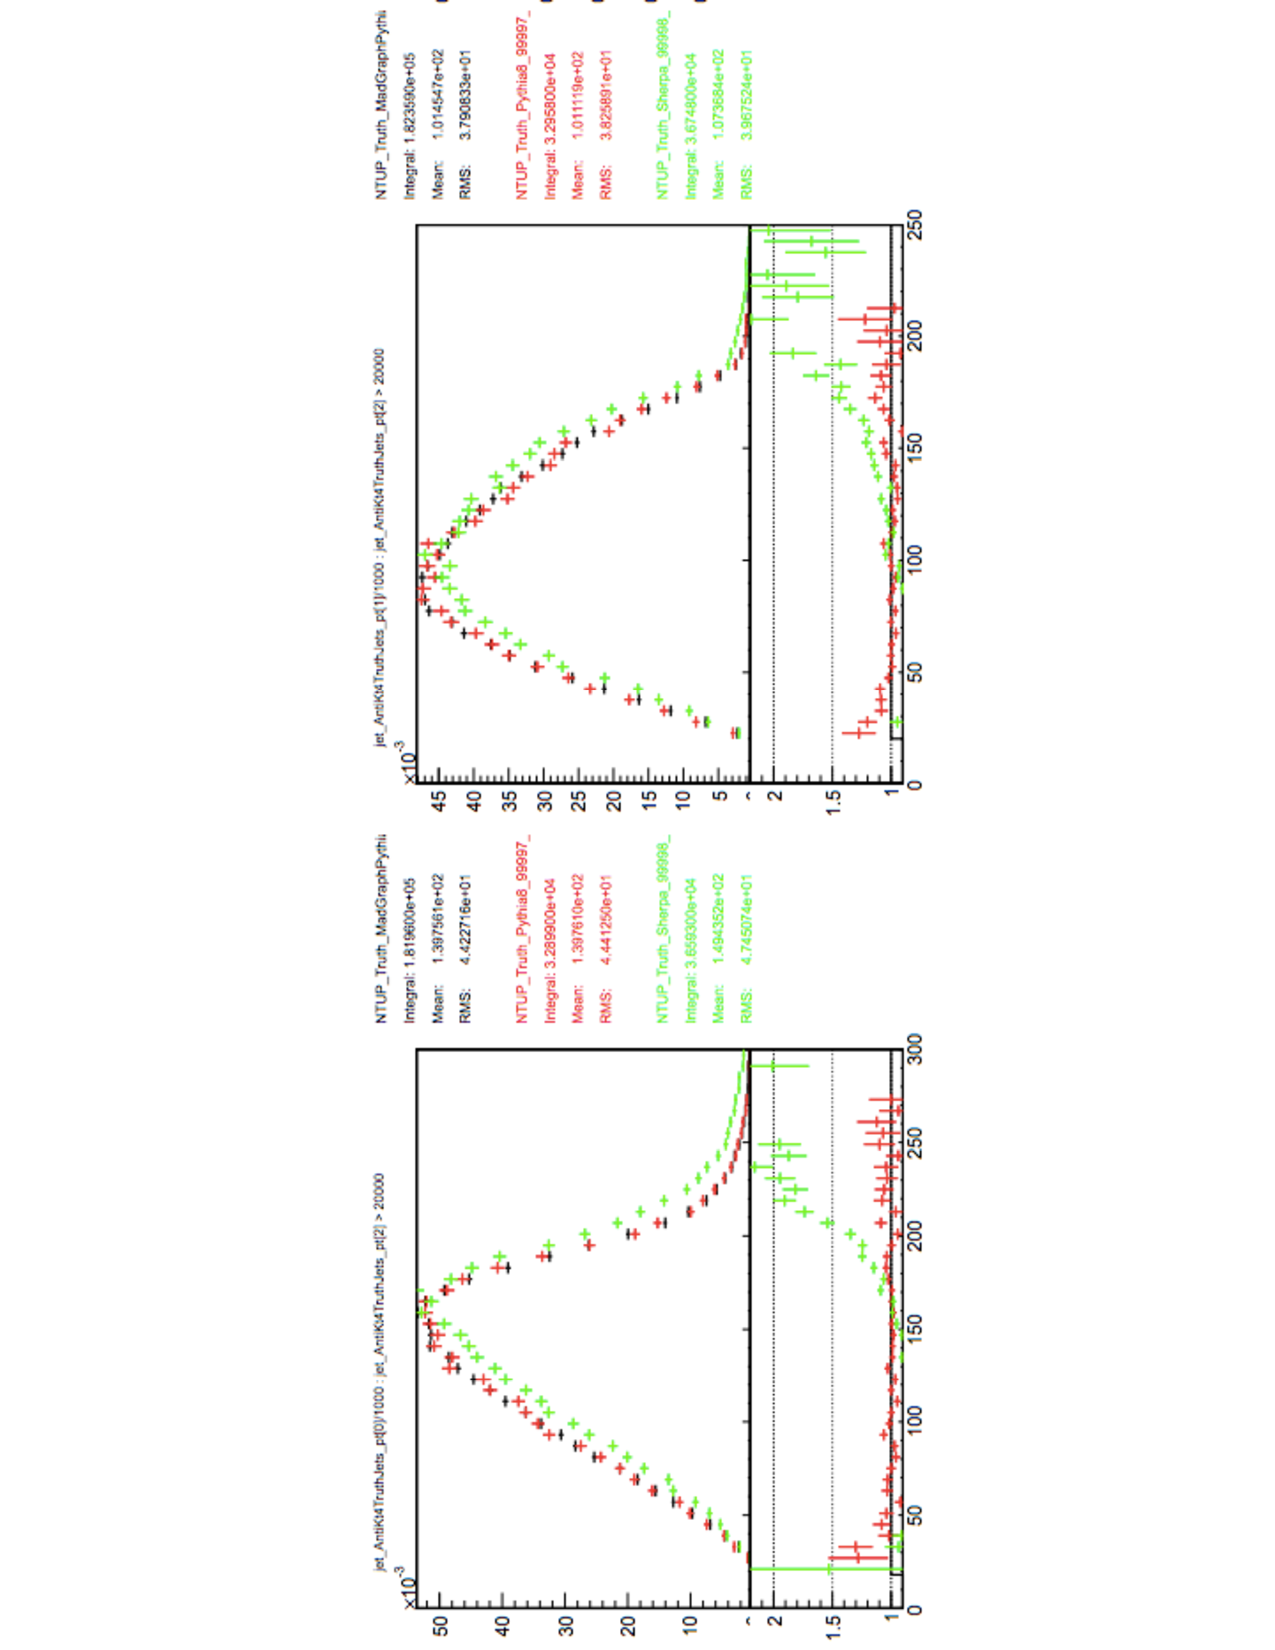
\includegraphics[width=0.7\textwidth, angle=270]{MonteCarlo/figures/sig_gen_compare.pdf}
  \caption{$p_T$ distributions for the leading 2 jets for Pythia (red), Sherpa (green) and MadGraph (black).  
  Pythia and MadGraph show good agreement, while Sherpa jets are systematically harder.  \label{fig:sig_gen_compare}}
\end{figure}
\begin{figure}
  \center
  \includegraphics[width=0.7\textwidth]{MonteCarlo/figures/mbb_sherpa_pythia_madgraph.pdf}
  \caption{$m_{bb}$ distributions for the leading 2 jets for Pythia (red), Sherpa (green) and MadGraph (black).  
  Pythia and MadGraph show good agreement, while the Sherpa $m_{bb}$ distribution is higher and more sharply peaked. \label{fig:mbb_sherpa_pythia_madgraph}}
\end{figure}

In order to understand if this disagreement was caused, at least in part, by
mixing up the associated $b$-jets and the Higgs daughter jets, we switched the Sherpa
generation process to $bH\rightarrow b\tau\tau$ and examined the properties of the
Higgs itself in addition to the jets (or $\tau$ leptons) in the event.  The $p_T$ and 
$\eta$ distributions of the di-tau (i.e. Higgs) system are in Figures~\ref{fig:di_tau_eta}
and~\ref{fig:di_tau_pt}, and the $m_{\tau\tau}$ distribution is in Figure~\ref{fig:di_tau_mass}.



\begin{figure}
  \center
  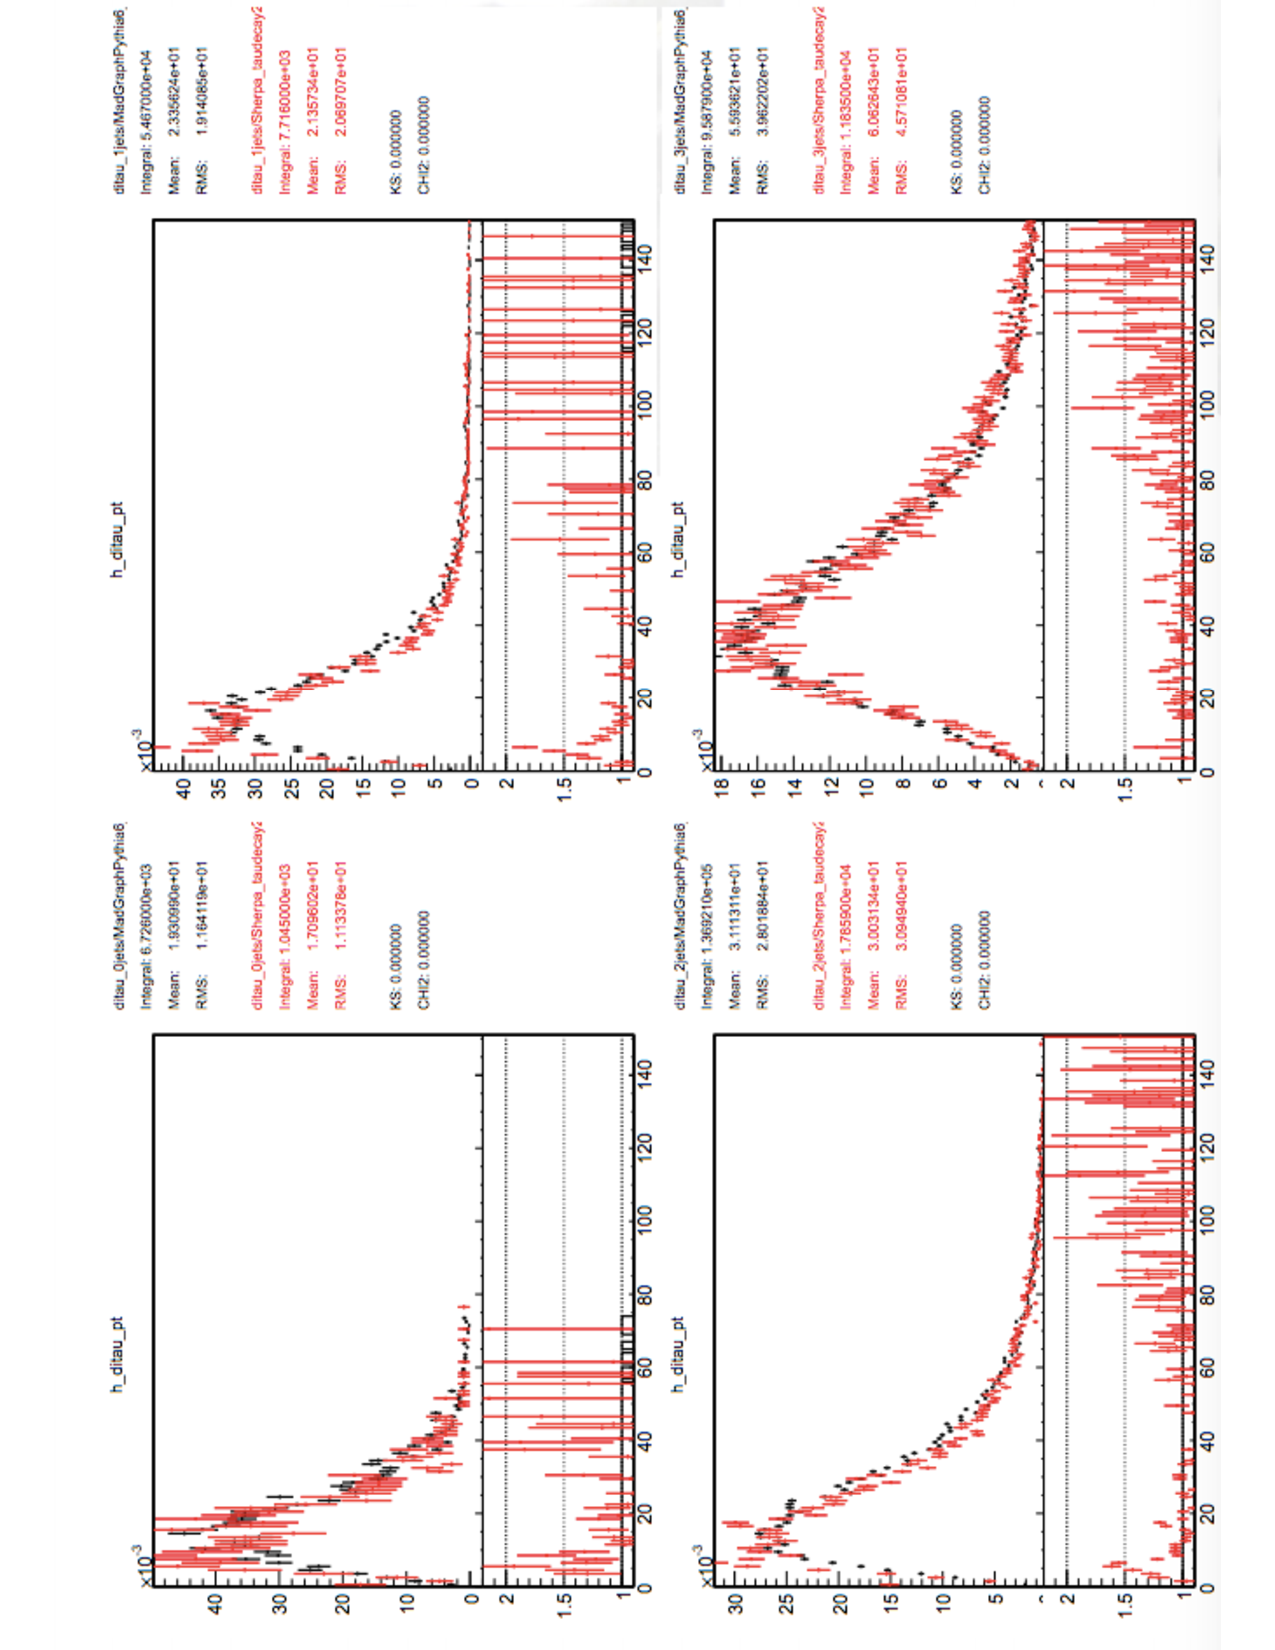
\includegraphics[width=0.8\textwidth, angle=270]{MonteCarlo/figures/di_tau_pt.pdf}
  \caption{$p_T$ distributions for the 2 $\tau$ leptons for Sherpa (red) and Madgraph (black) for 0 (upper
  left), 1 (upper right), 2 (lower left), and 3 (lower right) jets per event. 
  The Higgs system is more forward (larger $|\eta|$ in Sherpa than in MadGraph.  \label{fig:di_tau_pt}}
\end{figure}
\begin{figure}
  \center
  \includegraphics[width=0.8\textwidth, angle=270]{MonteCarlo/figures/di_tau_eta.pdf}
  \caption{$\eta$ distributions for the 2 $\tau$ leptons for Sherpa (red) and Madgraph (black) for 0 (upper
  left), 1 (upper right), 2 (lower left), and 3 (lower right) jets per event. 
  The Higgs system is more forward (larger $|\eta|$ in Sherpa than in MadGraph.  \label{fig:di_tau_eta}}
\end{figure}
\begin{figure}
  \center
  \includegraphics[width=0.8\textwidth, angle=270]{MonteCarlo/figures/di_tau_mass.pdf}
  \caption{$m_{\tau\tau}$ distributions for the 2 $\tau$ leptons for Sherpa (red) and Madgraph (black) for 0 (upper
  left), 1 (upper right), 2 (lower left), and 3 (lower right) jets per event. 
  The Higgs system is more forward (larger $|\eta|$ in Sherpa than in MadGraph.  \label{fig:di_tau_mass}}
\end{figure}


Upon more careful examination, we found that Sherpa segfaulted when trying to produce 
$gg\rightarrow H$ Feynman diagrams and so those diagrams had been excluded from
the initial production, although
an exchange with the Sherpa authors \footnote{most notably Stefan Hoche and Steffen 
Schumann, who we thank for their helpful advice throughout this analysis} provided 
a patch that enabled $gg\rightarrow H$ diagrams.  To understand
if the absence $gg\rightarrow H$ diagrams in Sherpa were responsible for the disagreement
with MadGraph, we generated samples of MadGraph events with and without the $gg\rightarrow H$
diagrams and compared the $p_T$ and $\eta$ of the Higgs system (Figure ~\ref{fig:ggH}).
The Higgs $p_T$ and $\eta$ do not show a bias depending on whether the gluon diagrams
are included or not, so it is not clear that including the gluon diagrams in Sherpa would
resolve the disagreement that we see. 

\begin{figure}
  \center
  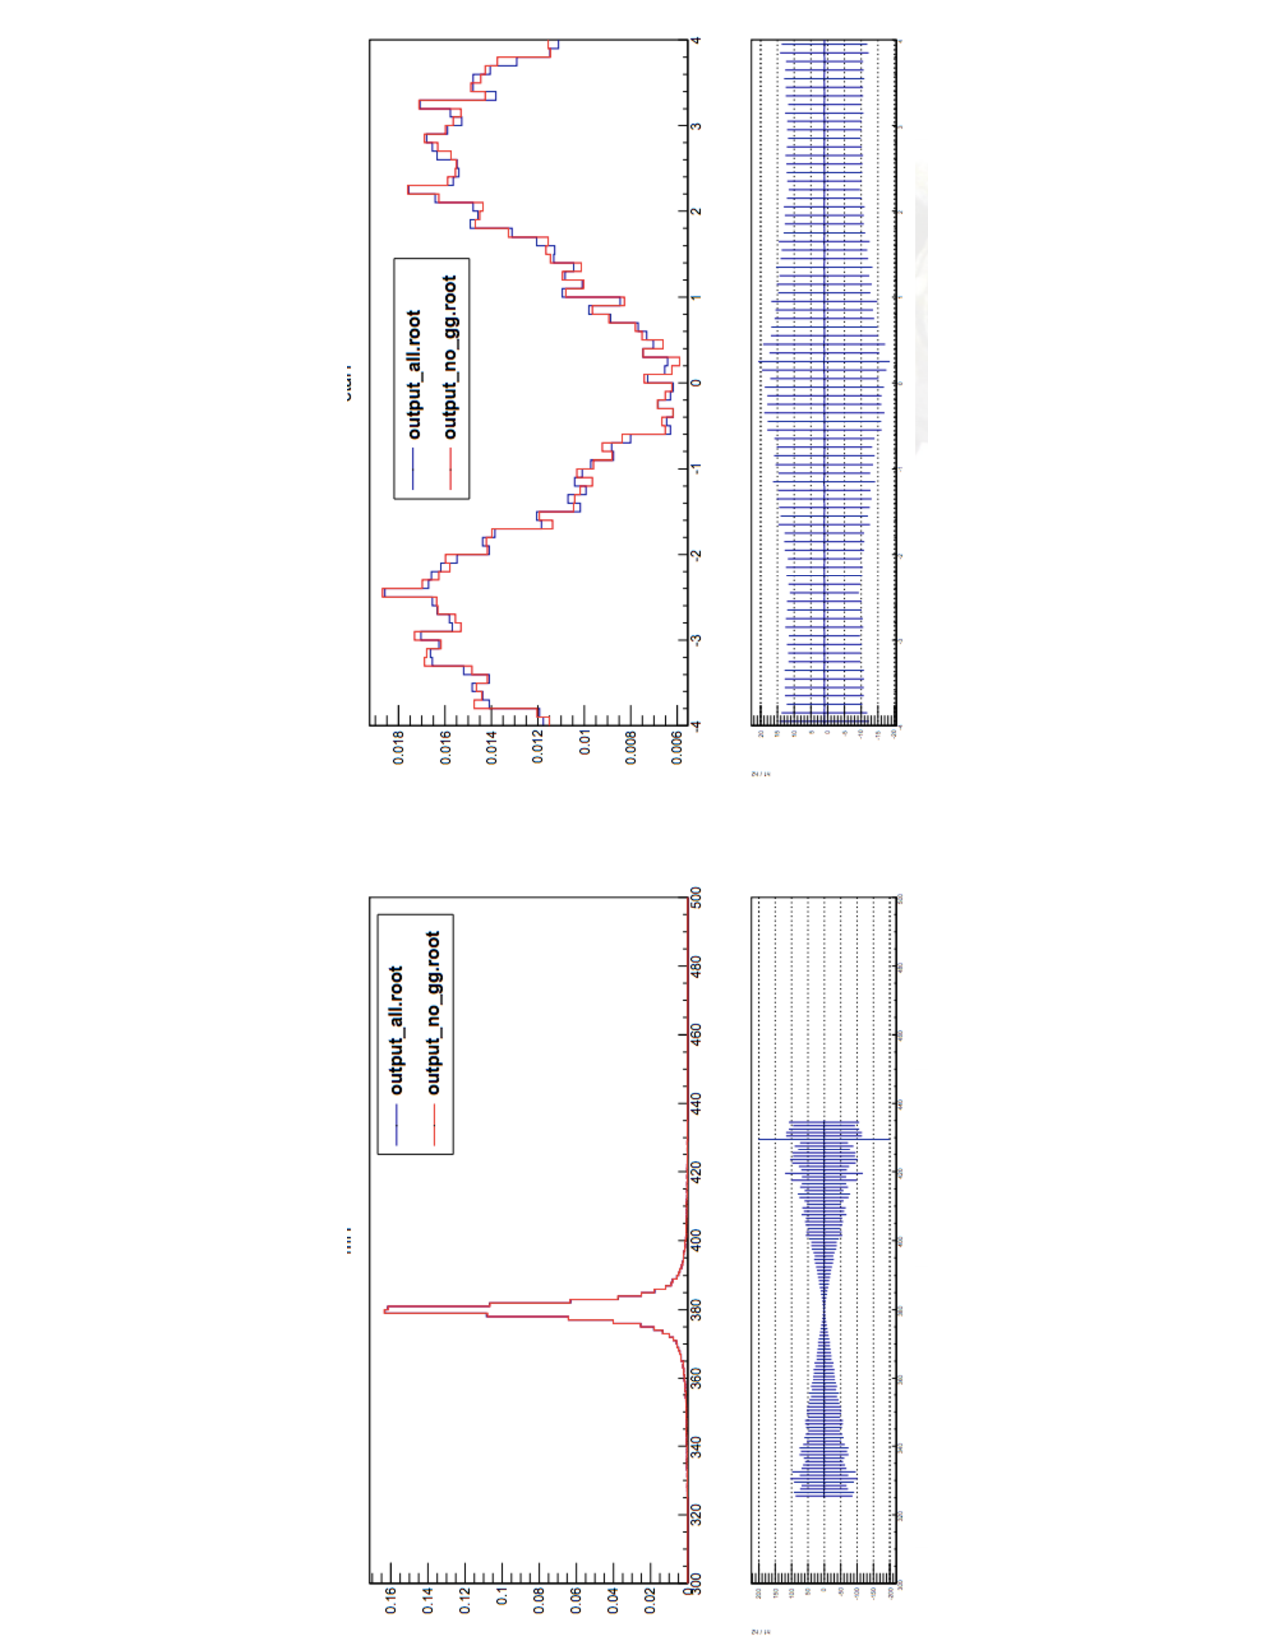
\includegraphics[width=0.8\textwidth, angle=270]{MonteCarlo/figures/ggH.pdf}
  \caption{$\eta$ distributions for the leading 2 jets for Sherpa (red) and Madgraph (black) for 0 (upper
  left), 1 (upper right), 2 (lower left), and 3 (lower right) jets per event. 
  The Higgs system is more forward (larger $|\eta|$) in Sherpa than in MadGraph.  \label{fig:ggH}}
\end{figure}




\section{Background}
\subsection{QCD Background}
Although QCD is the largest and most important background in this analysis, fully modeling 
it with QCD has some important drawbacks, which motivates our decision to use a 
mostly data-driven background estimation method.  That having been said, MC can 
still be a very valuable tool for making basic estimates and validating assumptions. 

There are two major types of QCD background in this analysis: first, when 
there is one or more mistakenly $b$-tagged light flavor or charm jets, 
which we call \textit{reducible} because, at least in theory, 
it could be identified and isolated/removed; and second, the \textit{irreducible} 
QCD background in which three real $b$-jets are present in the final 
state but without the intermediate resonance of the Higgs.  Both sources of background are 
expected to be significant but generally require different MC generation strategies.



\subsubsection{QCD Multijet}
The ATLAS QCD multijet MC collection is dataset is generated using Pythia8 \cite{Pythia8}.  
One of the major challenges of a truly inclusive sample like this one is that 
low-$p_T$ jets dominate the production cross section but generally have 
very low efficiency through the triggers or analysis cut flows, which is addressed by 
generating events several times with filtering applied based on the $p_T$ 
of the leading jet.  This leads to a distinctive ``slice'' structure to 
the sample, where 8 different slices are generated, each with a different $p_T$ 
range for the leading jet, and then the slices are knitted together with different 
relative weights to produce an inclusive spectrum with high statistics at all $p_T$ values.  

\begin{table}[h]
 \begin{center}
\caption{Hard subprocesses simulated in the bb QCD MC event sample, along with their cross sections. Here
$j=u,\bar{u},d,\bar{d},s,\bar{s},g$
\label{tab:qcd_mc_parameters}}
    \begin{tabular}{l r r r r r} \hline \hline
    Index & Dataset ID & $p_T$ Range& Cross Section (nb)& Filter Eff   & N Events \\ \hline
    0     &  147910    & 0-20        &  72850000.0       &      0.98557 & 1000000 \\
    1     &  147911    & 20-80       &  72850000.0       &   0.00012909 & 999996  \\
    2     &  147912    & 80-200      &     26359.0       &    0.0039901 & 999893 \\
    3     &  147913    & 200-500     &      544.18       &     0.001222 & 914584 \\
    4     &  147914    & 500-1000    &      6.4453       &   0.00070839 & 999773 \\
    5     &  147915    & 1000-1500   &    0.039739       &    0.0021516 & 957565 \\
    6     &  147916    & 1500-2000   &   0.0004161       &    0.0046773 & 299929 \\
    7     &  147917    & 2000+       &  4.0636e-05       &     0.014595 & 299988 \\
    \end{tabular}
  \end{center}
\end{table}

ATLAS has a high-statistics inclusive QCD MC sample that is used primarily in 
this analysis for understanding the QCD background from 
mistagged charm and light flavor (Table~\ref{tab:qcd_mc_parameters}.  Since 
the sample is inclusive, there is no filtering on the flavor of the jets 
that are produced (although there is dedicated effort to have high-$p_T$ 
jets simulated with adequate statistics) and the vast majority of jets are light or 
charm jets.  As a result, while we use this sample to estimate the 
efficiency and flavor composition of the QCD production in ATLAS as a whole, a 
particularly important background (QCD $bbb$) is virtually absent from this sample.


\subsubsection{$b$-Enriched QCD Multijet}
\label{sec:bb_qcd_mc}
\textbf{note: all distributions will be replaced with the higher-stats sample when
it is skimmed/processed}
Since the inclusive QCD Multijet samples are inadequate for understanding the $bb$ and 
$bbb$ MC backgrounds, we generate a dedicated sample that undergoes filtering to 
enrich it in heavy flavor.  This sample is generated using Sherpa 1.4.3 
\cite{Sherpa} and detector simulation is done with AFII.  This sample 
starts with a 5-flavor PDF that assumes massive $b$-quarks and 
2, 3 or 4 final state partons; then a filter is applied that 
requires that the leading 2 partons in the event be true $b$-quarks 
as well as requiring that the leading parton have a $p_T$ 
of at least 55 GeV (the latter requirement helps keep an acceptable efficiency when 
the sample is passed through the trigger and offline cuts).


%---------------------------------------
\begin{table}[h]
 \begin{center}
\caption{Hard subprocesses simulated in the bb QCD MC event sample, along with their cross sections. Here
$j=u,\bar{u},d,\bar{d},s,\bar{s},g$}
\label{tab:sherpa_subprocesses}
    \begin{tabular}{l|r} \hline \hline
   subprocess      & cross section (pb)\cr \hline

$jj\rightarrow b\bar{b}jj$ & 58531 \cr
$jj\rightarrow b\bar{b}j$ & 33411 \cr
$bj\rightarrow bjj \ \ +\ \  \bar{b}j\rightarrow \bar{b}jj$ & 22147 \cr
$bj\rightarrow bjjj \ \ +\ \  \bar{b}j\rightarrow \bar{b}jjj$ & 16282 \cr
$bj\rightarrow b j \ \ +\ \  \bar{b} j\rightarrow \bar{b} j$ & 12135 \cr
$jj\rightarrow b\bar{b}$ &  1672 \cr
$cj\rightarrow c b\bar{b}j \ \ +\ \  \bar{c} j\rightarrow \bar{c}  b\bar{b}j$ & 1602 \cr
$bj\rightarrow b b\bar{b}j \ \ +\ \  \bar{b} j\rightarrow \bar{b}  b\bar{b}j$ & 997 \cr
$jj\rightarrow b\bar{b}c\bar{c}$ &  776 \cr
$cj\rightarrow c b\bar{b} \ \ +\ \  \bar{c} j\rightarrow \bar{c}  b\bar{b}$ & 681 \cr
$bj\rightarrow b b\bar{b} \ \ +\ \  \bar{b} j\rightarrow \bar{b}  b\bar{b}$ & 387 \cr
$jj\rightarrow b\bar{b}b\bar{b}$ &  376 \cr
$b\bar{c}\rightarrow b\bar{c}j \ \ +\ \  \bar{b} c\rightarrow \bar{b} cj$ & 206 \cr
$bc\rightarrow bcj\ \ +\ \  \bar{b}\bar{c}\rightarrow \bar{b} \bar{c}j$ & 194 \cr
$b\bar{c}\rightarrow b\bar{c}jj \ \ +\ \  \bar{b} c\rightarrow \bar{b} cjj$ & 143 \cr
$bc\rightarrow bcjj\ \ +\ \  \bar{b}\bar{c}\rightarrow \bar{b} \bar{c}jj$ & 136 \cr
$bc\rightarrow bc\ \ +\ \ \bar{b}\bar{c}\rightarrow \bar{b} \bar{c}$ & 122 \cr
$b\bar{c}\rightarrow b\bar{c} \ \ +\ \  \bar{b} c\rightarrow \bar{b} c$ & 121 \cr
$b\bar{b}\rightarrow b\bar{b}j$ & 62 \cr
$bb\rightarrow bbj\ \ +\ \  \bar{b}\bar{b}\rightarrow \bar{b} \bar{b}j$ & 53 \cr
$b\bar{b}\rightarrow b\bar{b}jj$ & 44 \cr
$bb\rightarrow bbjj\ \ +\ \  \bar{b}\bar{b}\rightarrow \bar{b} \bar{b}jj$ & 39 \cr
$b\bar{b}\rightarrow b\bar{b}$ & 37 \cr
$bb\rightarrow bb\ \ +\ \  \bar{b}\bar{b}\rightarrow \bar{b} \bar{b}$ & 30 \cr
\hline
   \end{tabular}
  \end{center}
\end{table}
%---------------------------------------



%-----------------------------------------------                     
\begin{figure}
  \center
  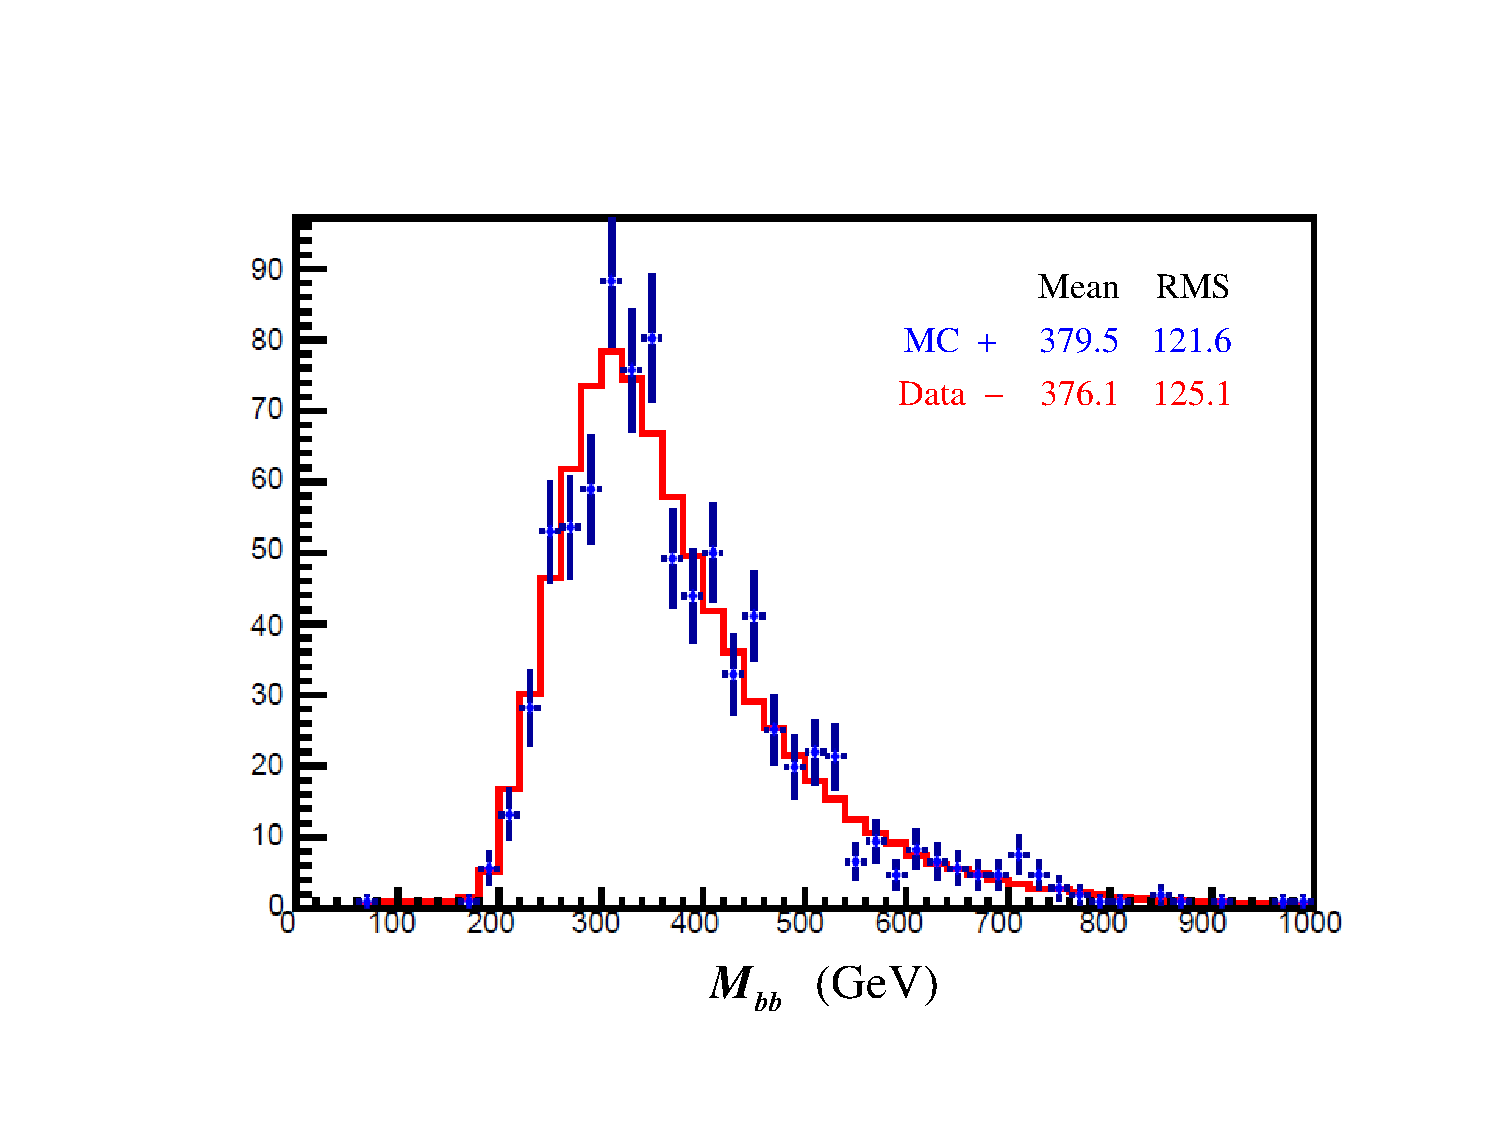
\includegraphics[width=0.70\linewidth]{MonteCarlo/figures/mbb_bbqcd_vs_data.pdf}
  \caption{Mass of the two leading jets in events passing all cuts except the
bbb, bbloose and bbanti classification.  Distributions for the 10,000 event bb QCD Monte Carlo validation sample
and a 2.2~fb$^{-1}$ luminosity data sample are shown.    \label{fig:mbb_bbqcd_vs_data}}
\end{figure}

\begin{figure}
  \center
  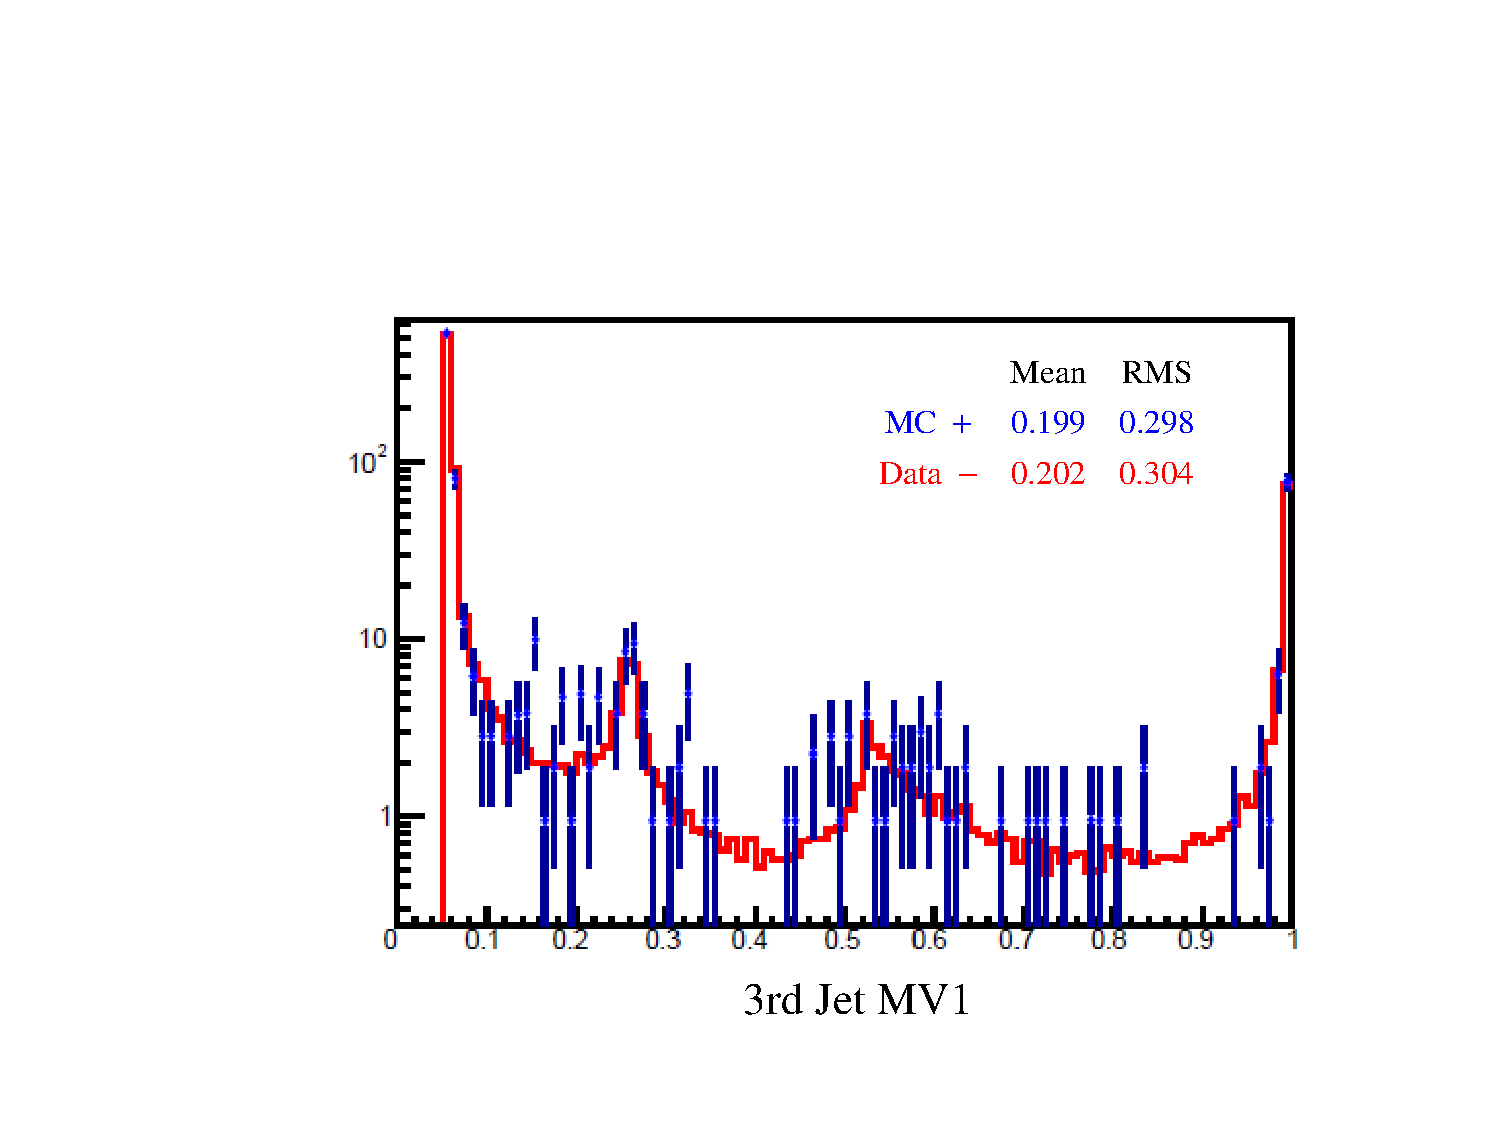
\includegraphics[width=0.70\linewidth]{MonteCarlo/figures/mv1_jet3_bbqcd_vs_data.pdf}
  \caption{The b-tag variable MV1 for the 3rd leading $p_T$ jet in events passing all cuts except the
bbb, bbloose and bbanti classification.     Distributions for the 10,000 event bb QCD Monte Carlo validation sample
and a 2.2~fb$^{-1}$ luminosity data sample are shown.    \label{fig:mv1_jet3_bbqcd_vs_data}}
\end{figure}




\begin{figure}
  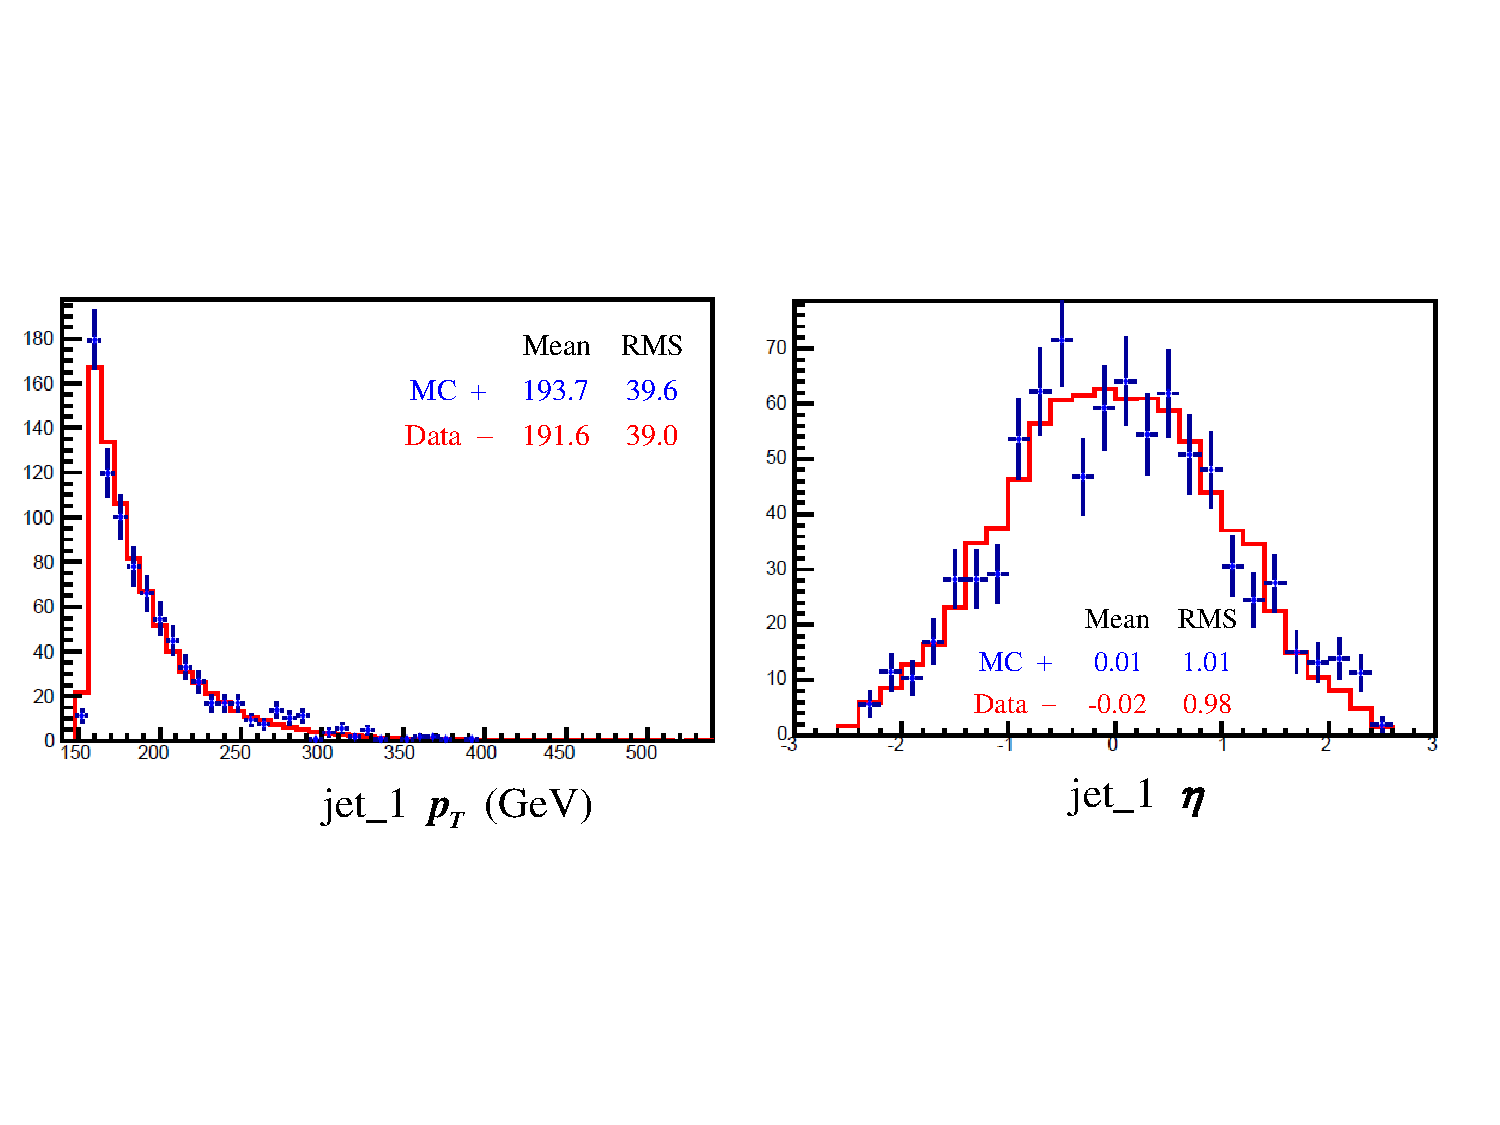
\includegraphics[width=0.85\linewidth]{MonteCarlo/figures/pt_eta_jet1_bbqcd_vs_data.pdf}
  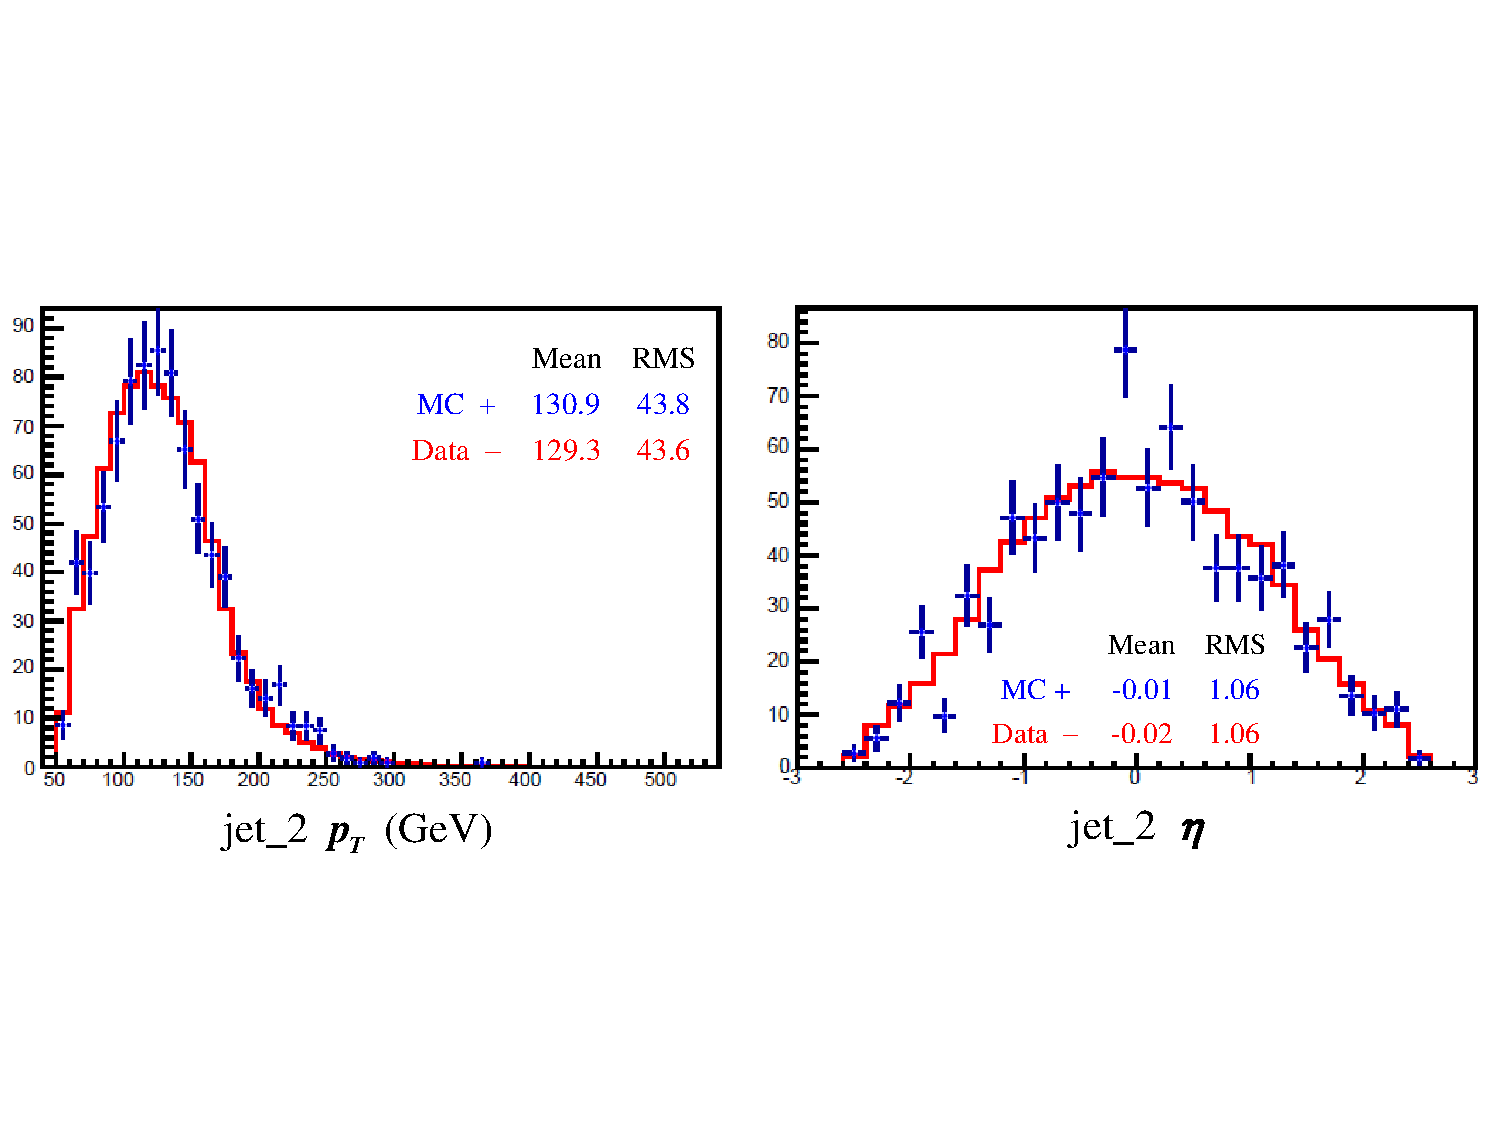
\includegraphics[width=0.85\linewidth]{MonteCarlo/figures/pt_eta_jet2_bbqcd_vs_data.pdf}
  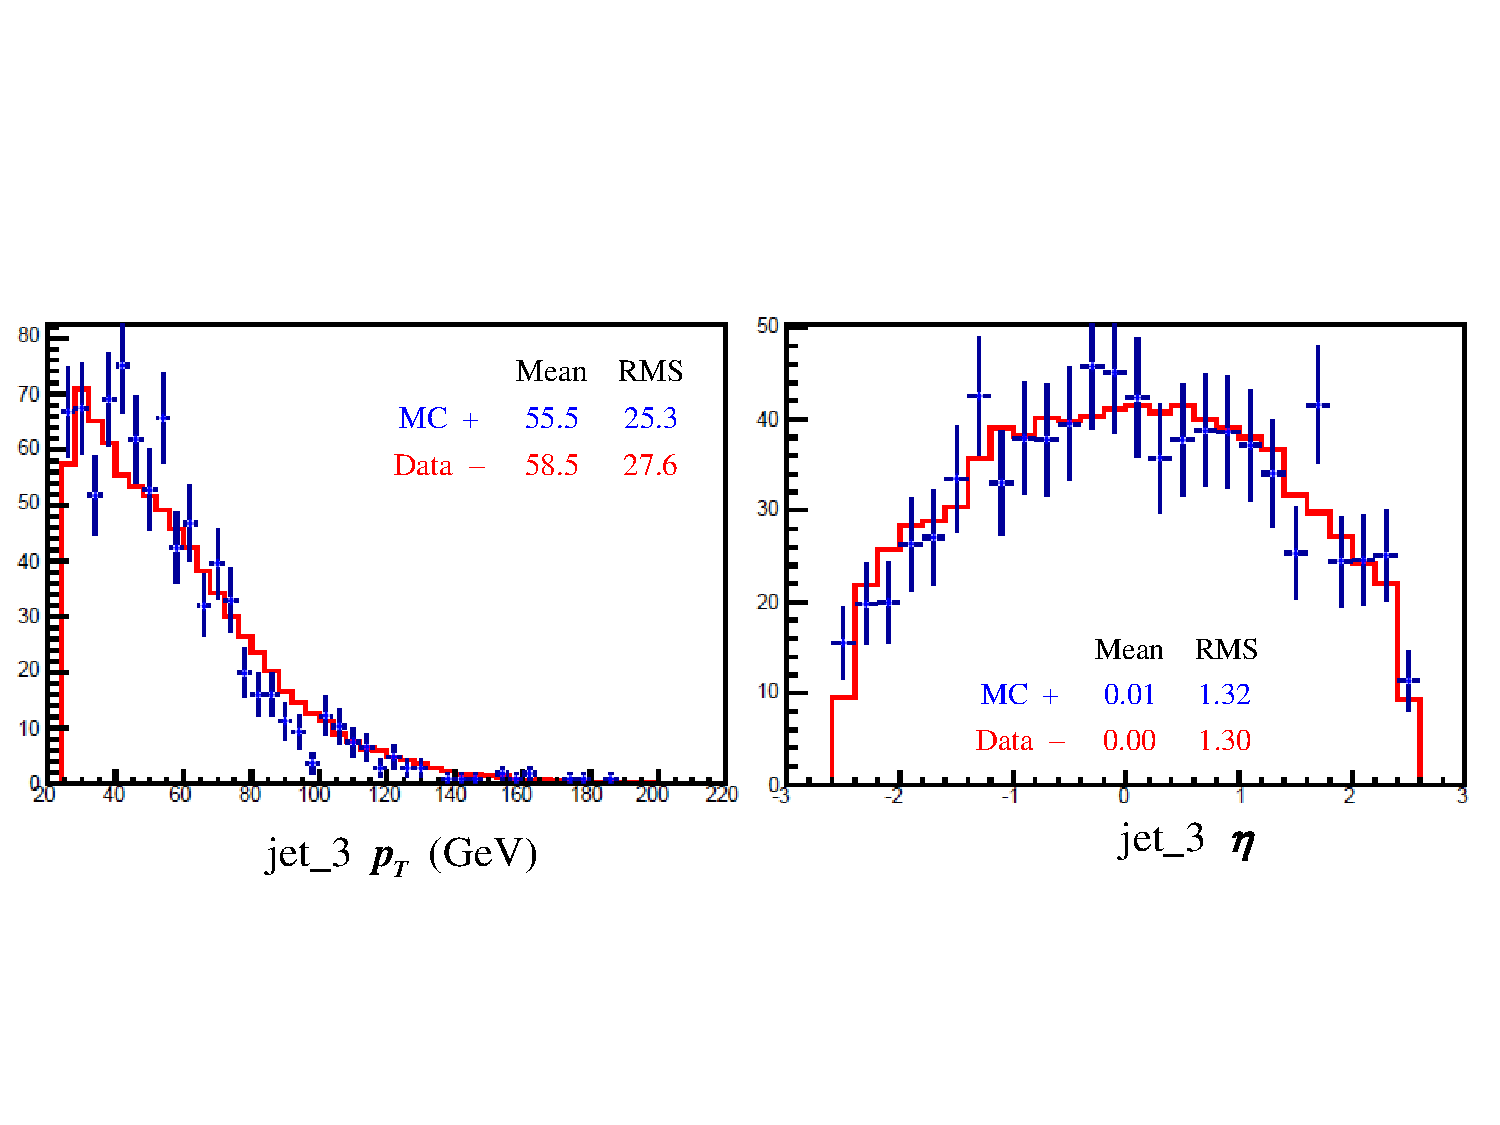
\includegraphics[width=0.85\linewidth]{MonteCarlo/figures/pt_eta_jet3_bbqcd_vs_data.pdf}
  \caption{$p_T$ and $\eta$ for the three leading $p_T$ jets in events passing all cuts except the
bbb, bbloose and bbanti classification.     Distributions for the 10,000 event bb QCD Monte Carlo validation sample                 
and a 2.2~fb$^{-1}$ luminosity data sample are shown.    \label{fig:pt_eta_bbqcd_vs_data}}                                          
\end{figure}                                                                                                                        
%-----------------------------------------------                     



%\subsection{Top Background}
%Top-antitop pairs decaying all-hadronically is the largest non-QCD background.  The sample generated
%to model this background is generated in Powheg and Pythia, with Tauola and Photos also used for
%handling tau leptons and photons.  In practice, $t\bar{t}$ is a minor background, both because
%of its small cross section relative to QCD and because in the high mass ranges most relevant for
%this search, it does not show any sigificant structure or $m_{bb}$ shape differences depending
%on the flavor of the third jet.
%
%
%\begin{table}
%   \caption{Parameters of the $t\bar{t}$ MC sample used in this analysis. \label{tab:ttbar_params} }
%    \begin{tabular}{ c c c c }
%    Dataset ID & Cross Section [nb] & Filter Efficiency & N Events \\
%    117050     & 0.21085        & 0.54298    & 99930891 \\
%    \end{tabular}
%\end{table}

%--------------------------------------------------------






